\begin{frame}
\frametitle{Precision determination of spin tune\,\textcolor{PineGreen}{\cite{PhysRevLett.115.094801}} I}

\begin{block}{Time-stamping events in each detector quadrant accurately:}
\begin{enumerate}
	\item Based on turn number $n$, \SI{100}{s} measurement interval split into turn intervals of $\Delta n = \SI{e6}{turns}$, each interval lasting $\approx \SI{1.3}{\second}$.
	\item  For all events, spin phase advance $\varphi_s = 2 \pi | \nu_s^\text{fix} |n $ calculated assuming certain fixed spin tune $\nu_s^\text{fix}$.
	\item Either map events into one full polarization oscillation in range $\varphi_s \in [0, 2\pi)$, or perform Fourier analysis of rates in detector $\Rightarrow$ determine  $\tilde \varepsilon$ and $\tilde \phi$ in 
	\begin{equation}
	\varepsilon(\varphi_s) = \tilde \varepsilon \sin(\varphi_s + \tilde \varphi)\,.
	\end{equation}
\end{enumerate}
\end{block}

\vspace{0.3cm}
\begin{columns}
	\column{0.45\textwidth}
	\centering 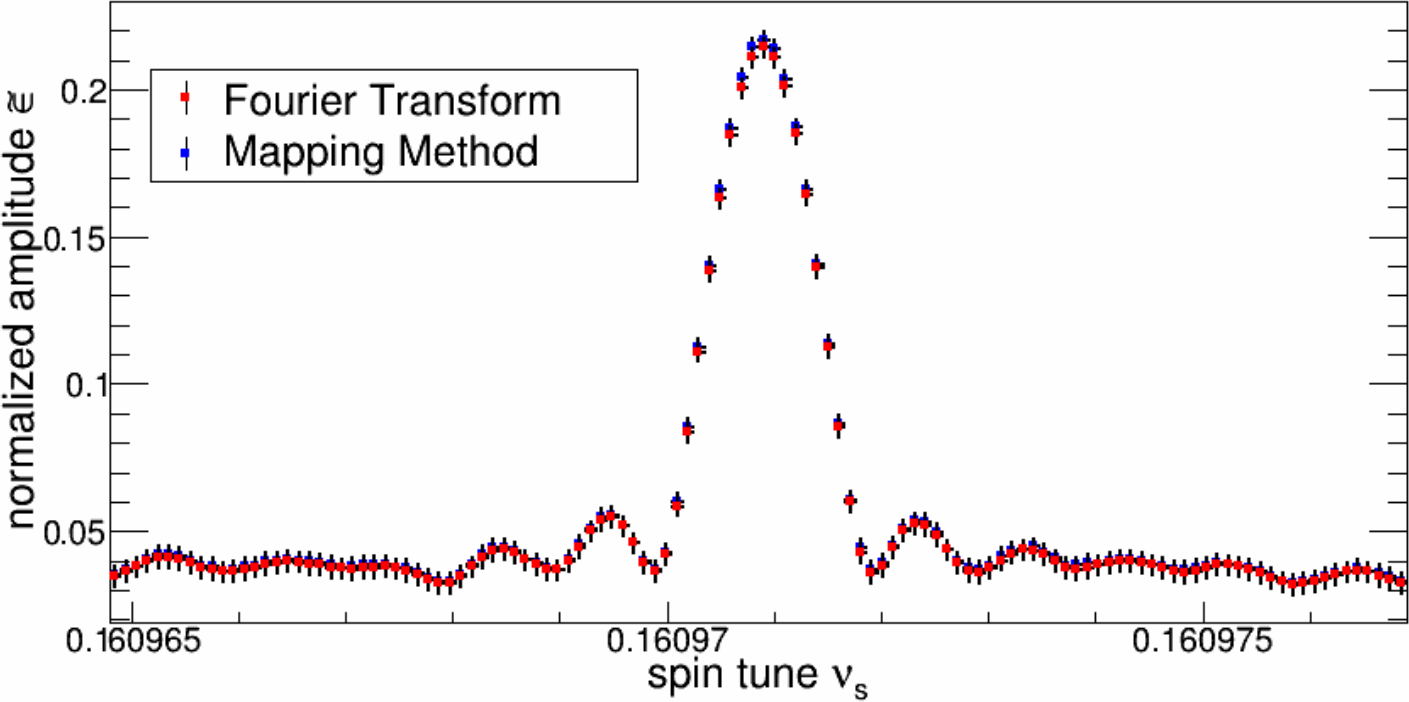
\includegraphics[height = 0.3\textheight]{spin-tune-spectrum.png} 
	\column{0.45\textwidth}  
	\centering 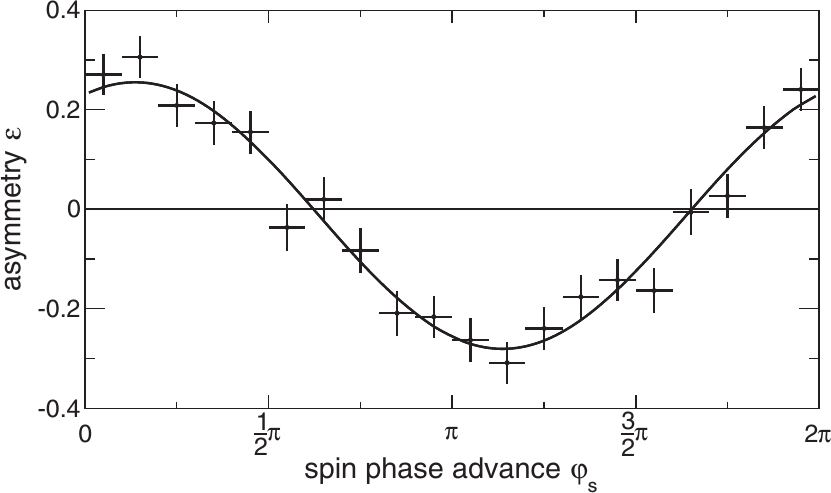
\includegraphics[height = 0.3\textheight]{phase-plot-spin-tune.png}
\end{columns}

\end{frame}